\begin{anexosenv}

\partanexos

\chapter{Protótipos elaborados no trabalho}\label{anexos}

\lstinputlisting[language=Python,caption={Protótipo em \textit{Python} para estudo do pacote {\code apt}.},label=proto_apt]{editaveis/prototipos/prototipo_apt.py} 
\cleardoublepage

\lstinputlisting[language=Python,caption={Protótipo do algoritmo de \textit{match} exato.},label=proto_exact]{editaveis/prototipos/exact.py}
\cleardoublepage

\lstinputlisting[language=Python,caption={Protótipo do algoritmo de \textit{Levenshtein}.},label=proto_leven]{editaveis/prototipos/protoLevenshtein.py}
\cleardoublepage

\lstinputlisting[language=Python,caption={Protótipo do algoritmo de \textit{Damerau-Levenshtein}.},label=proto_damerau]{editaveis/prototipos/protoDamerauLevenshtein.py}
\cleardoublepage

\lstinputlisting[language=Python,caption={Protótipo do algoritmo de \textit{Smith-Waterman}.},label=proto_smith]{editaveis/prototipos/protoSmith.py}
\cleardoublepage

% Texto do primeiro anexo.

\chapter{\nmu Figuras \nmu Extensas}\label{long_figures}

% \begin{figure}[h]
%   \centering
% 	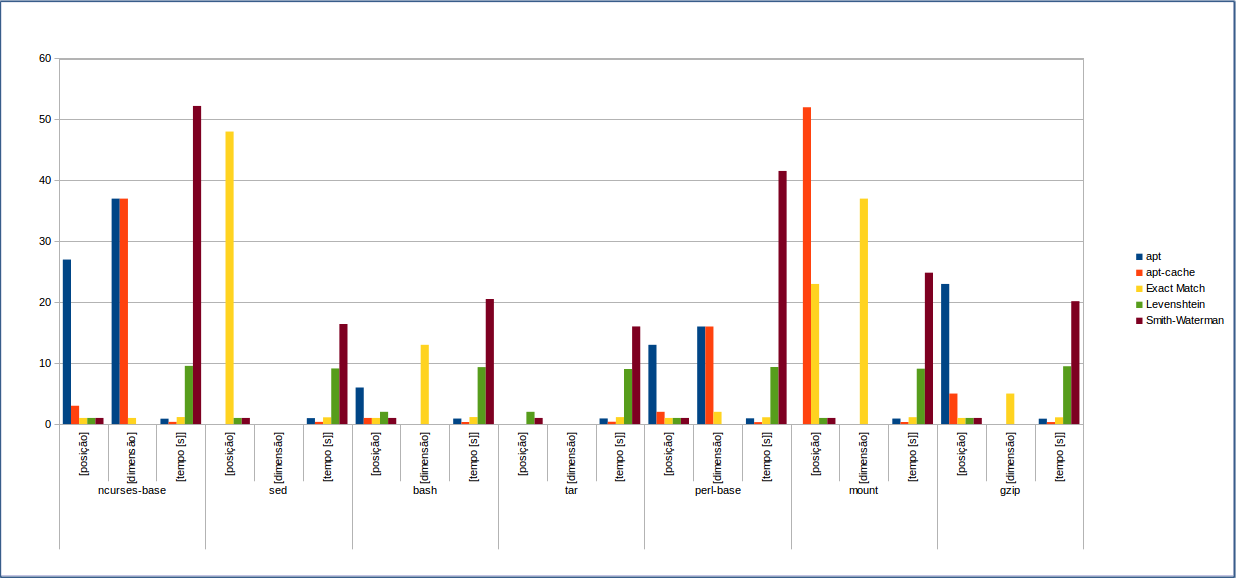
\includegraphics[width=0.7\textheight,angle=90]{figuras/grafico}
%   \caption{Amostra de comparação dos resultados}
%   \label{fig:figuras_grafico}
% \end{figure}
% \cleardoublepage

\begin{figure}[h]
  \centering
	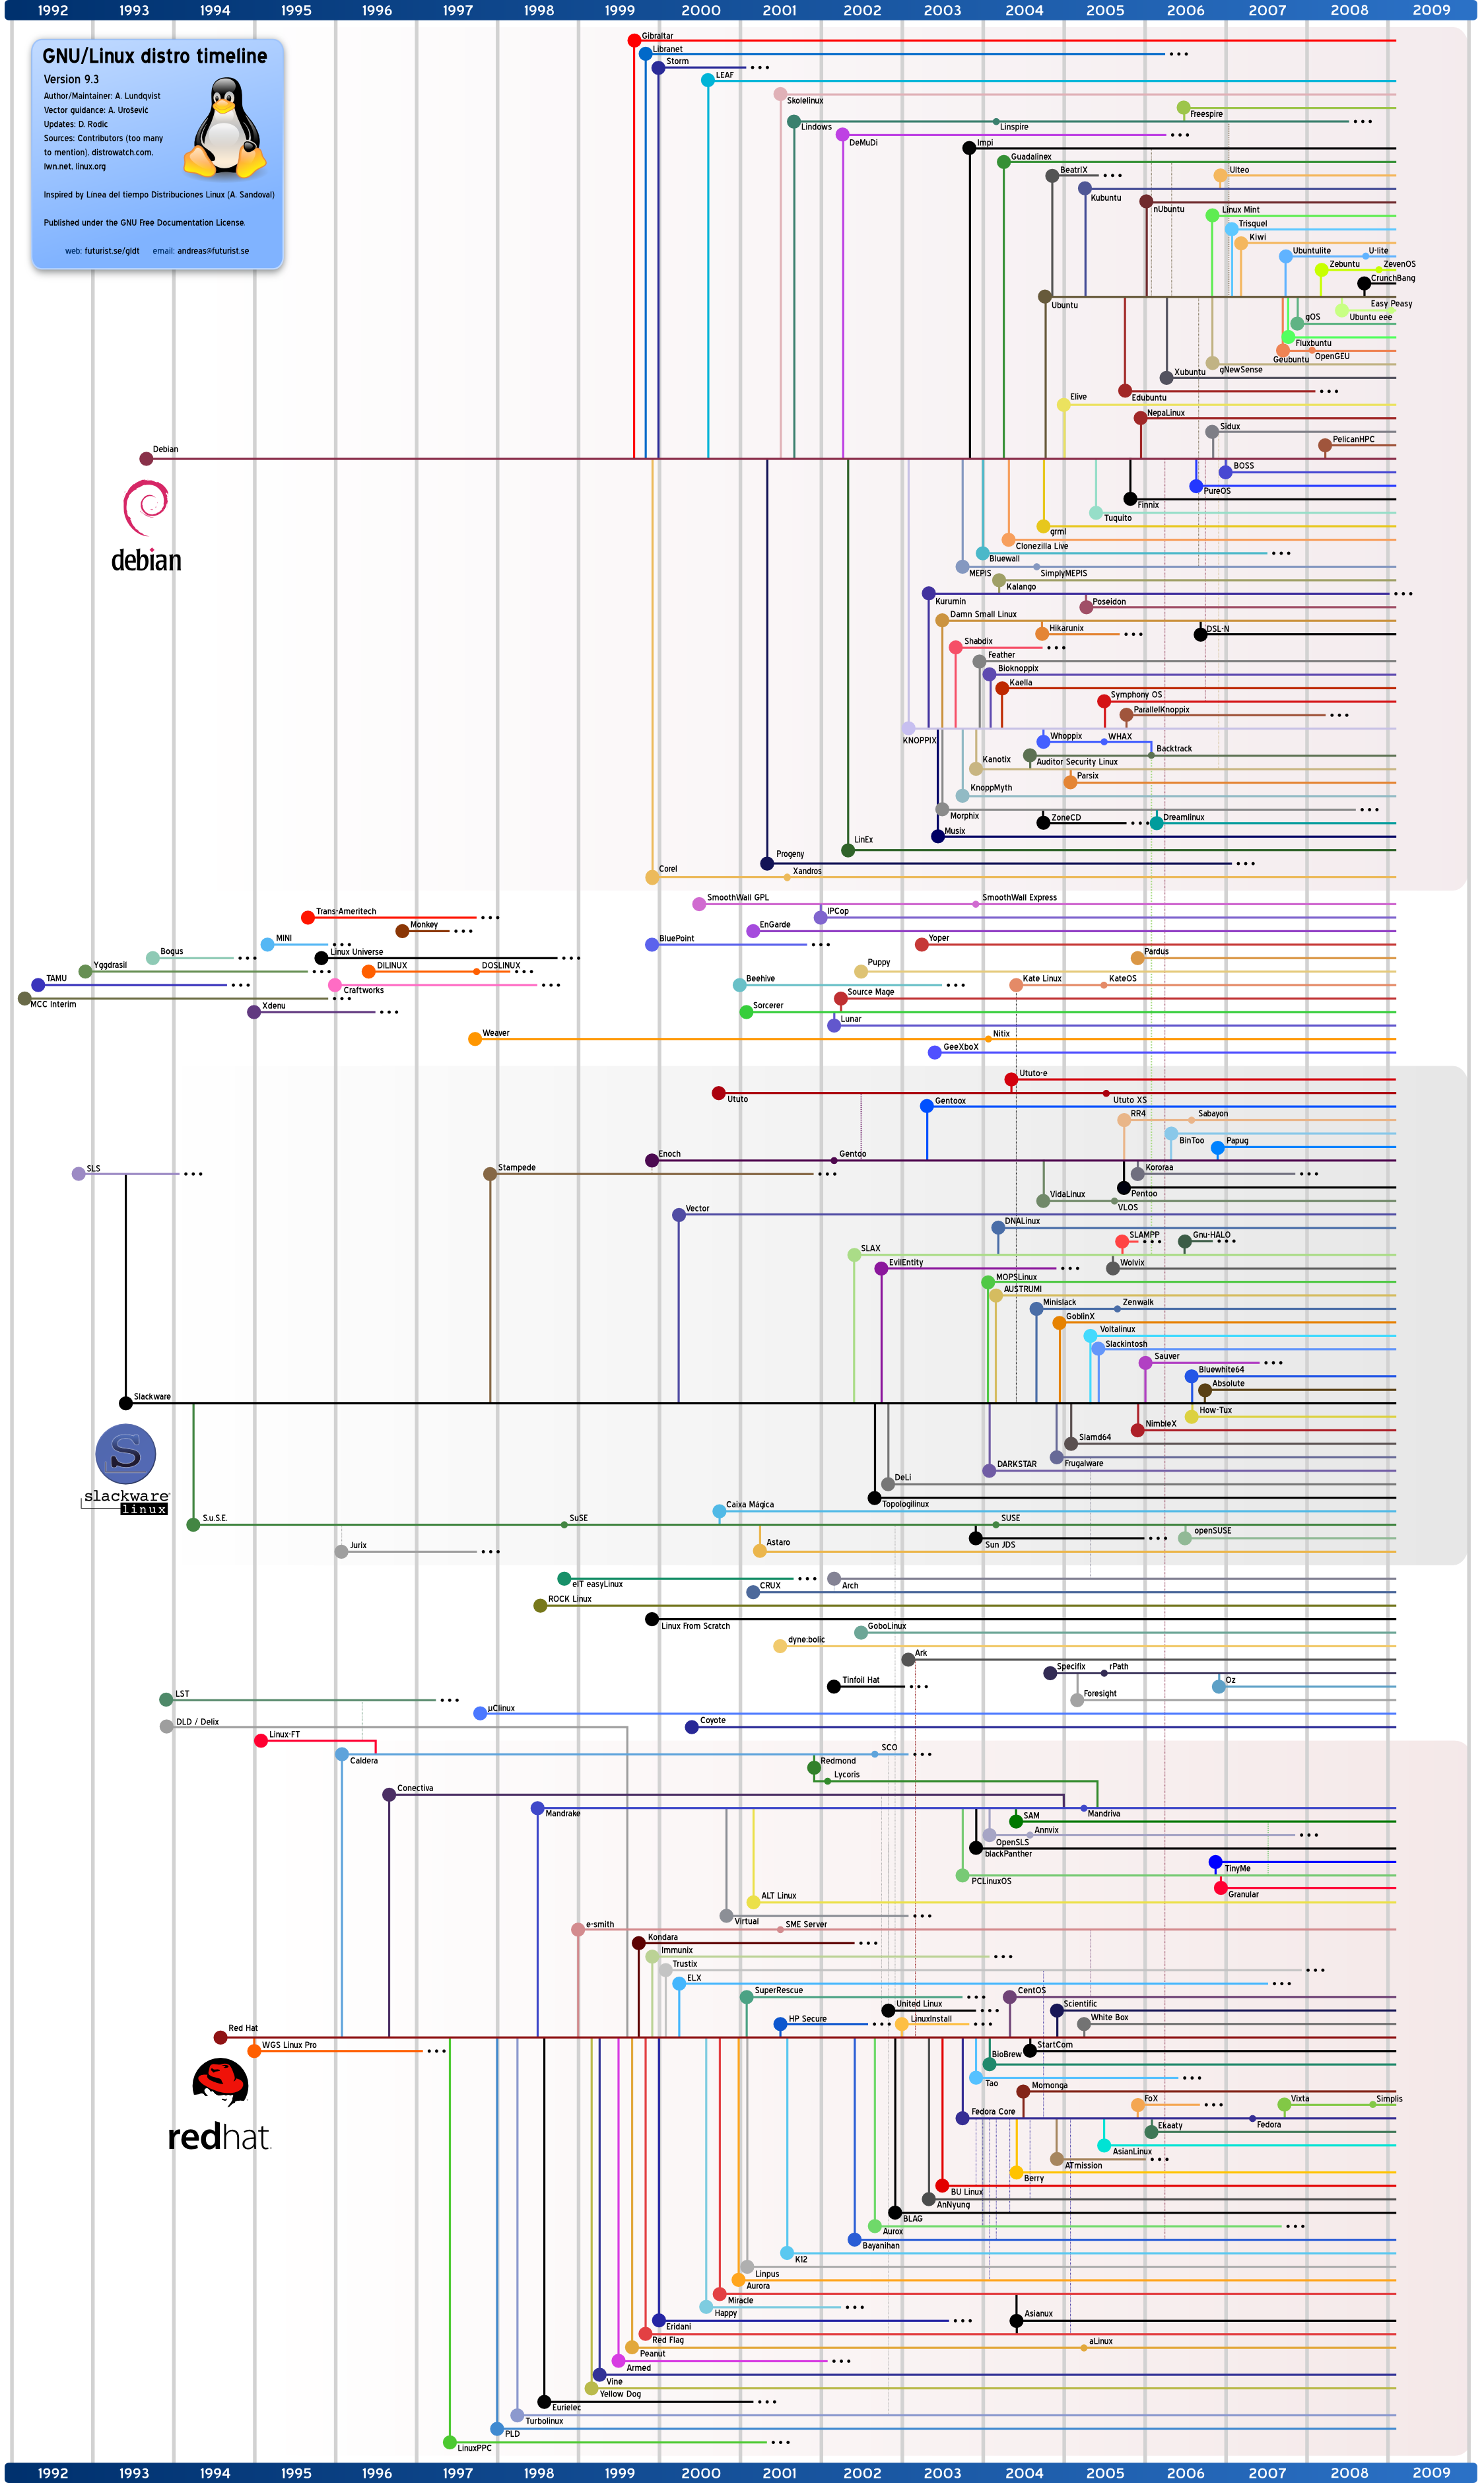
\includegraphics[width=0.78\textwidth]{figuras/linux-timeline-heranca}
  \caption{Heranças de algumas das distribuições Linux existentes hoje\protect\footnotemark.}
  \label{fig:figuras_linux_timeline_heranca}
\end{figure}
\footnotetext{\label{note:figuras_linux_timeline_heranca}\textbf{Fote:} \href{http://www.linux-es.org/files/distribuciones_en_el_tiempo.png}{www.linux-es.org}}

% Texto do segundo anexo.

\end{anexosenv}

